\documentclass[11pt,dvipdfm]{article}
%\documentclass[11pt]{article}

\usepackage{deauthor, times,graphicx}

\usepackage{url}


\usepackage{hyperref}
\usepackage{color} 
\usepackage{colortbl}

\usepackage{xcolor}
\definecolor{Gray}{gray}{0.91}

%%For algorithms
\usepackage{algorithm2e}
\usepackage{algpseudocode}
% https://shantoroy.com/latex/how-to-write-algorithm-in-latex/
\newcommand\mycommfont[1]{\footnotesize\ttfamily\textcolor{blue}{#1}}
\SetCommentSty{mycommfont}
\SetKwInput{KwInput}{Input}                % Set the Input
\SetKwInput{KwOutput}{Output}              % set the Output




\usepackage{listings}
\usepackage{booktabs}
\usepackage{multirow}
\usepackage{amssymb}
\usepackage{subfig}
\usepackage{graphicx}
\usepackage{stfloats}
\usepackage{mathtools}
\usepackage{adjustbox}
\usepackage{tabularx}
\usepackage{caption}
\usepackage{amsmath}
\usepackage{version}


\let\oldemptyset\emptyset
\let\emptyset\varnothing

\newcommand{\bits}{\{0,1\}}
\newcommand{\mc}[1]{\mathcal{#1}}
\newcommand{\pick}{\leftarrow}
\newcommand{\negl}{\mathsf{negl}}
\newcommand{\mb}[1]{\mathbf{#1}}
\newcommand{\mbb}[1]{\mathbb{#1}}
\newcommand{\al}[1]{\mathsf{#1}}
\newcommand{\secp}{\lambda}





\usepackage{natbib}
\bibliographystyle{abbrvnat}
\setcitestyle{numbers,open={[},close={]}} %Citation-related commands


\begin{document}

\title{Differential Privacy with Fine-Grained Provenance: Opportunities and Challenges}

\author{
  Xi He\\
    University of Waterloo\\
      \texttt{xi.he@uwaterloo.ca}
  \and
        Shufan Zhang\\
  University of Waterloo\\    \texttt{shufan.zhang@uwaterloo.ca}
}

%https://tc.computer.org/tcde/data-engineering-bulletin/tcde-bulletin-author-instructions/

% Differential Privacy with Fine-grained  Provenance for Databases: Opportunities and Challenges

%https://arxiv.org/pdf/2004.08887

\maketitle

\begin{abstract}
Online crowdsourcing platforms have proliferated over the last few years and cover a number of important domains, these platforms include from worker-task platforms such Amazon Mechanical Turk, worker-for-hire platforms such as TaskRabbit to specialized platforms with specific tasks such as ridesharing like Uber, Lyft, Ola etc.
An increasing proportion of human workforce will be employed by these platforms in the near future.
The crowdsourcing community has done yeoman's work in designing
effective algorithms for various key components, such as incentive design, task assignment and quality control. Given the increasing importance of these crowdsourcing platforms,
it is now time to design mechanisms so that it is easier to evaluate the effectiveness of these platforms. Specifically, we advocate developing benchmarks for crowdsourcing research.

Benchmarks often identify important issues for the community to focus and improve upon.
This has played a key role in the development of research domains as diverse as
databases and deep learning.
We believe that developing appropriate benchmarks for crowdsourcing will ignite further innovations.
However, crowdsourcing -- and future of work, in general -- is a very diverse field
that makes developing benchmarks much more challenging.
Substantial effort is needed that spans across developing benchmarks for
datasets, metrics, algorithms, platforms and so on.
In this article, we initiate some discussion into this important problem and
issue a call-to-arms for the community to work on this important initiative.
\end{abstract}


\section{Introduction}

Differential privacy (DP)~\cite{dwork2006calibrating} emerged in 2006 as a groundbreaking concept for protecting individual privacy in data analysis. DP offers a powerful privacy-preserving approach by mathematically ensuring that data releases reveal minimal information about any single person. This has led to the development of numerous DP mechanisms and systems like PINQ~\cite{mcsherry2009pinq}, FLEX~\cite{johnson2018towards}, PrivateSQL~\cite{kotsogiannis2019privatesql}, GoogleDP~\cite{amin2022plume}, and Chorus~\cite{johnson2020chorus}.
However, despite its theoretical elegance and strong privacy guarantees, DP's practical deployments lag behind its potential. While a few pioneering cases exist, such as the 2020 US Census disclosure~\cite{abowd2018census,hawes2020census}, widespread adoption remains limited. Companies like Amazon, Snowflake, Google, LinkedIn, Uber, and Apple, and startups like Tumlut Labs and Transcend are exploring DP in data management products or statistical learning scenarios~\cite{amazon_DP,snowflake_DP,google_DP_big_query,wilson2020differentially,houssiau2022google_map,rogers2020linkedin,DingKY17microsoft_DP, openDP,tumult, transcend}, but these integrations are often experimental and face challenges in production environments~\cite{tang2017privacy,GadottiHAM22apple_DP_attack,yu2022thwarting}, suggesting a divergence between theory and practice.

In theory, DP relies on a privacy budget, represented by the parameters $(\epsilon,\delta)$, which controls the overall privacy guarantee. By carefully injecting controllable noise, it can be proved that a mechanism can only reveal bounded information about any individual in a \textit{static} dataset, and thus, this mechanism satisfies the notion of DP. However, translating this theory into practical systems presents several challenges. 
First, even with a simple use case that only focuses on the \emph{central DP} setting\footnote{Assuming the existence of a \emph{trusted} curator runs a (data analytics) system with DP guarantees for a curated sensitive dataset.}, the system has to interact with private data and data analysts and has to maintain the system budget at least correctly and faithfully. 
Some systems resort to large or frequently reset budgets~\cite{rogers2020linkedin,amazon_DP}, which may jeopardize long-term privacy. Second, DP systems often assume static datasets. However, real-world data can be dynamic, integrating information from various sources~\cite{nicolas2023cohere} and undergoing regular updates~\cite{growingdb18}. The individuals in the dataset may have different privacy awareness~\cite{jorgensen2015personalized}.
These complexities require additional considerations to maintain privacy guarantees. Third, DP systems need to cater to analysts with varying levels of privacy expertise. Non-expert analysts may struggle to interpret noisy results or choose the most appropriate DP mechanism for their queries~\cite{ge2019apex}, especially for complex queries, like nested subqueries or batched workloads~\cite{nissim2007smooth,dong2021residual}. As a result, implementations of the DP system can fail to deliver an optimized privacy-utility trade-off or the expected privacy guarantees.


Recent DP systems have addressed one specific challenge mentioned above by tracking fine-grained information such as the data blocks~\cite{LecuyerSVG019sage,nicolas2023cohere} or the noise used for previous queries~\cite{mazmudar2022cache,zhang2022DProvSQL}. 
Inspired by these works, we propose a broader approach to building usable end-to-end DP systems by leveraging the data provenance framework in databases~\cite{cheney2009provenance}, in which tracing and propagating \textit{proper provenance metadata} turns out to be useful for understanding queries, integrating data, and debugging inconsistencies. Similarly, in DP systems, we envision privacy provenance --- metadata that tracks the DP mechanisms and benefits the users of the systems. 
 
In this work, we analyze different components of a DP system and explore how proper provenance metadata can offer benefits, including improved user understanding, enhanced utility optimization, and dynamic privacy management. We start with three types of privacy provenance: \textit{why-DP-provenance}, which explains the private/noisy outputs to the data analysts; \textit{how-DP-provenance}, which uses metadata for tighter privacy in running DP mechanisms; and \textit{where-DP-provenance}, which tracks privacy budget consumption over dynamic data sources to satisfy different resolutions of privacy definitions. While the concept of privacy provenance is a recent development~\cite{dprovdb}, the idea of leveraging additional data structures in DP algorithm design has been explored in prior work~\cite{johnson2020chorus,mcsherry2009pinq,gaboardi2016psi,NanayakkaraB0HR22visualizing}. We surveyed all the relevant DP works in our privacy provenance framework and provided discussion in this direction.  
Note that our characterization of privacy provenance in this work is not meant to be exhaustive. We hope this work stimulates further exploration and discussion in developing more usable and optimized systems for DP. 
This work also aims to complement existing visions on DP (including recent surveys~\cite{cummings2024advancing_DP_survey,near2021differential}). 
By introducing a system-oriented perspective through the lens of privacy provenance, we hope to pave the way for the development of more usable and optimized DP systems in the future.


\stitle{Article Roadmap.}
The remainder of this article is organized as follows.
Section 2 summarizes the preliminaries of differential privacy and provenance in databases.
In Section 3, we provide a systematic view of the complexity of the DP systems and propose a taxonomy of fine-grained privacy provenance.
We survey several systems that feature the usages of fine-grained privacy provenance in Section 4 and discuss challenges and future directions in Section 5.
We conclude this article in Section 6.




\section{Background}

We introduce and summarize the related definitions of differential privacy.
Next, we introduce the necessary preliminaries for differential privacy and provenance in databases.

\subsection{Definition of Differential Privacy}

\begin{definition}[Differential Privacy \cite{dwork2006calibrating}]

We say that a randomized algorithm $\mc{M}: \databasedom \rightarrow  \mc{O}$ 
satisfies $(\epsilon, \delta)$-differential privacy (DP), if for any two
neighbouring databases $(D,D')$ that differ in only 1 tuple, 
and $O\subseteq \mc{O}$, we have
$$
\Pr[\mc{M}(D) \in O] \leq e^\epsilon \Pr[\mc{M}(D') \in O] + \delta.
$$
\end{definition}

\begin{definition}[Global Sensitivity]
For a query $q: \mathcal{D} \rightarrow \mathbb{R}^d$ 
the $\ell_2$ global sensitivity of this query is 
$$
\Delta q = \max_{D, D': d(D,D') \leq 1} \| q(D) - q(D') \|_2,
$$ 
where $d(\cdot, \cdot)$ denotes the number of tuples that $D$ and $D'$ differ and $\| \cdot \|_2$ denotes the $\ell_2$ norm. If we replace the $\ell_2$ norm with $\ell_1$ norm, then we obtain the $\ell_1$ sensitivity $\Delta_1 q$.
\end{definition}



\stitle{Basic DP Mechanisms.} The most basic DP mechanisms are the Laplace and Gaussian mechanisms, injecting Laplace and Gaussian noises, respectively, into the query answers, which are explained below.

\begin{definition}[Laplace Mechanism~\cite{dwork2014algorithmic}]
    Given a numerical query $q: \mathcal{D} \rightarrow \mathbb{R}^d$, the Laplace mechanism outputs $\mathcal{M}(D) = q(D) + \eta$  where 
$\eta \sim {Lap} \left( b \right)^d$ where ${Lap} \left( b \right)^d$ is a vector of $d$ i.i.d. samples from a Laplace distribution with scale $b$. If $b=\Delta_1 q/\epsilon$, then the Laplace mechanism preserves $(\epsilon, 0)$-DP.
\end{definition}

\begin{definition}[Gaussian Mechanism~\cite{dwork2014algorithmic}]
\label{def:standarad_gaussian_mech}
Let $\epsilon \in (0, 1)$. 
Given a numerical query $q: \mathcal{D} \rightarrow \mathbb{R}^d$, for constant $c > \sqrt{2\ln (1.25/\delta)}$, the Gaussian mechanism adds the noise vector $(\eta_1, \eta_2, \dots, \eta_d)$ to the query answer $q(D)$, where $\eta_i$ are i.i.d. random variables drawn from the Gaussian distribution $\mc{N}(0, \sigma^2I)$ with $\sigma > c \Delta q / \epsilon$.
The Gaussian mechanism is $(\epsilon, \delta)$-differentially private.
\end{definition}

The standard Gaussian mechanism \cite{dwork2014algorithmic} has the limitation that it can only be used in a high privacy regime, where the privacy parameter $\epsilon$ should be within the range of $(0, 1)$.
Balle and Wang \cite{BW18analytic} propose an improved mechanism, namely the analytic Gaussian mechanism, overcoming this limitation in the standard Gaussian mechanism.
We give the definition of analytic Gaussian mechanism below for completeness, while skipping the details of the mechanism does not affect understanding this article.

\begin{definition}[Analytic Gaussian Mechanism \cite{BW18analytic}]
\label{def:analytic_gaussian}
Given a query $q : \mathcal{D} \rightarrow \mathbb{R}^{d}$, the analytic Gaussian mechanism $\mathcal{M}(D) = q(D) + \eta$  where 
$\eta \sim {\mc{N}} \left( 0, \sigma^2 I \right)$ 
is $(\epsilon, \delta)$-DP if and only if 
$$
\Phi_{\mc{N}} \left( \frac{\Delta q}{2 \sigma} - \frac{\epsilon \sigma}{\Delta q} \right)
    - e^{\epsilon} \Phi_{\mc{N}} \left( - \frac{\Delta q}{2 \sigma} - \frac{\epsilon \sigma}{\Delta q} \right) 
    \leq \delta,
$$
where $\Phi_{\mc{N}}$ denotes the cumulative density function (CDF) of Gaussian distribution. In this mechanism, the Gaussian variance is determined by $\sigma = \alpha \Delta q / \sqrt{2\epsilon}$ where $\alpha$ is a parameter determined by $\epsilon$ and $\delta$~\cite{BW18analytic}.
\end{definition}
 

\stitle{Privacy Composition Theory.}
Differential privacy enjoys the nice property of being compositional.
Running a DP mechanism multiple times is also DP, but with a higher privacy cost.
One can, therefore, build complex mechanisms by composing basic DP mechanisms using the following composition theorems.


\begin{theorem}[Sequential Composition \cite{dwork2014algorithmic}]
\label{thm:dp_seq_composition}
Given two mechanisms $\mc{M}_1: \databasedom \rightarrow  \mc{O}_1$ and $\mc{M}_2: \databasedom \rightarrow  \mc{O}_2$, such that $\mc{M}_1$ satisfies $(\epsilon_1, \delta_1)$-DP and $\mc{M}_2$ satisfies $(\epsilon_2, \delta_2)$-DP.
The combination of the two mechanisms $\mc{M}_{1, 2}: \databasedom \rightarrow  \mc{O}_1 \times \mc{O}_2$, which is a mapping $\mc{M}_{1, 2}(D) = (\mc{M}_1(D), \mc{M}_2(D))$, is $(\epsilon_1+\epsilon_2,\delta_1+\delta_2)$-DP.
\end{theorem}

\begin{theorem}[Parallel Composition~\cite{mcsherry2009pinq}]
    Let a mechanism $\mc{M}: \mc{D} \rightarrow \mc{O}$ be $(\epsilon,\delta)$-DP. If $D_1, \dots, D_n \in \mc{D}$ are $n$ arbitrary disjoint sets of databases and $X = D_1 \cup \dots \cup D_n$, the release of mechanism output sequence $\mc{M}(D_1), \dots, \mc{M}(D_n)$ satisfies $(\epsilon,\delta)$-DP. 
\end{theorem}

\begin{theorem}[Post Processing \cite{dwork2014algorithmic}]
\label{thm:dp_post_processing}
For an $(\epsilon, \delta)$-DP mechanism $\mc{M}$, applying any arbitrary function $f$ over the output of $\mc{M}$, that is, the composed mechanism $f \circ \mc{M}$, satisfies $(\epsilon, \delta)$-DP.
\end{theorem}

\subsection{Provenance in Databases}

Provenance (sometimes also called lineage or pedigree) in databases~\cite{cheney2009provenance} studies the origin or history of the data through a high-level structured computation (e.g., data transformation or query execution) in its lifecycle. By recording more metadata through annotation~\cite{BunemanKT02annotations} or additional data structure (e.g., semiring)~\cite{GreenKT07provenance_semiring,GreenT17provenance_semiring}, data management systems can explain the relationships on how data items in the output (e.g., a tuple produced) depend on (various) source/input (e.g., multiple relational tables).
The most common provenance models are ``why-'', ``how-'', and ``where-'' provenances, aim to explain, respectively, \emph{why} a particular tuple appears in the output~\cite{BunemanKT01where-prov}, \emph{how} an output tuple is processed and derived~\cite{GreenKT07provenance_semiring}, and \emph{where}, precisely, an output tuple is originated in the sources according to the computation~\cite{BunemanKT01where-prov}.
Provenance information is useful for understanding the query behavior, data processing steps, and scientific workflows, and thus critical in auditing the integrity, reproducibility, and reliability of data in many scenarios~\cite{cheney2009provenance}.

The relationship between provenance and data privacy has received increasing attention~\cite{PanSR23provenance_sec_privacy,DavidsonKRSTC11prov_privacy,DavidsonKMPR11provenance,DeutchFGM21optimizing_privacy_utility_provenance,Pappachan2022tattletale,PappachanZHM23}. This line of research focuses on the potential privacy risks associated with tracking provenance information, particularly for sensitive data. Researchers explore how revealing provenance details could leak information and investigate techniques to minimize such risks. This might involve suppressing specific parts of provenance queries or hiding certain intermediate data while still achieving desired privacy guarantees.
Other recent work~\cite{WuTD22provenance} highlights how provenance can be used for maintaining and versioning machine learning models to mitigate privacy attacks towards the models.



\section{Privacy Provenance Overview}
This section explores how provenance information can be leveraged to enhance the effectiveness of DP systems. We introduce the concept of \emph{DP provenance}, a systematic approach to capture and utilize provenance to support DP systems. We propose a new taxonomy that categorizes existing work based on the type and granularity of the provenance considered. We then delve into how different types of provenance can be used to improve various aspects of DP systems.

\subsection{DP System Model: A Provenance Perspective}
\label{sec:dpsystem}
Every data system that integrates DP has to record and track some additional metadata, compared to that without DP.
We start with a simple, hypothetical system with DP to show the most basic functionalities and the coarsest privacy provenance tracking provided by it.
We then lay out the different entities/components of a DP system that motivate the need for finer-grained privacy provenance or additional provenance features.

\stitle{A (Hypothetically) Basic DP System.}
Consider running a DP system in the central setting, where a \emph{trusted data curator} maintains a protected database $D$.
The data curator sets up a finite \emph{system-wise or global privacy budget} to bound the overall extent of information disclosure \emph{over this database}.
(A group of) untrusted data analyst(s) would like to query the private database $D$.
Each incoming query from a data analyst specifies a \emph{per-query privacy budget} that indicates the amount of budget they would like to spend on this particular query. 
The DP system uses \textit{a fixed mechanism} (e.g., the Laplace mechanism) to answer this query, and subtracts the per-query privacy budget from the global budget.
The system rejects a query if the remaining global budget is not sufficient for this query; it stops processing queries once the global privacy budget is fully depleted.

This basic system can only support limited queries (that could be na\"ively answered through one fixed mechanism). 
Almost every DP system that researchers implement in literature is more complicated than it.
Even though, the basic system has to track the privacy loss in terms of the per-query privacy budget and the global budget consumption\footnote{Indeed, in real-world implementations which lack careful management, DP can rapidly become excessively restrictive so that service providers have to set up a large (or even infinite) global budget, which has been shown to attacks~\cite{tang2017privacy}.
}, which is the simplest example of privacy provenance.
This oversimplified setting overlooks the complexity of a real-world DP system.
Next, we will provide a view of the complexity of system designs for real-world DP systems.

\stitle{The Complexity of DP Systems.}
The design of a DP system greatly depends on the users's role, interest, and expertise levels in this system. First, the data analysts (who are the queries or the programmers) of a DP system have no direct access to the data. They care for the accuracy of the query results and how many queries they can interact with the system. Ideally, if the data analysts have the full domain knowledge of DP and how the system works, then they can understand the DP programs supported by the systems and trace the necessary meta information for optimizing their interested queries. If not, they may not be able to specify the privacy budget correctly and understand the noisy outputs.
A usable DP system in practice is expected to accommodate the needs of both types of data analysts. 
It should explain the noisy output to DP novices and provide modularized APIs for DP experts to program their own tasks.

Second, the data curators are responsible for setting up the data input for the programs and allocating privacy budgets among different analysts.
The basic DP system makes several assumptions to simplify the privacy analysis.
It assumes that the database is static (i.e., not subject to updating), and each row in the database corresponds to a single individual.
In addition, the privacy analysis is rigidly enforced at the entire table level, and the protection is uniform across every row in the database.
In real-world use cases, however, the underlying database is often under dynamic changing and has the hetergenous nature that not every part of the data is equally sensitive.
For example, new data analysts can keep opt-in, and their data will be merged into the private database when the system is running.
The data contributors may have different contributions to the database in terms of the number of rows.
They may also have personalized opinions or different privacy awareness regarding the protection of their data.
In such scenarios, keeping a single global privacy budget and simple privacy analysis at the table level is not sufficient to provide the desired level of privacy guarantees.
In addition, data analysts can have different trust or privilege levels when accessing the system. Tech companies, for example, need to query their users’ data for internal applications like anomaly detection. 
They also consider inviting external researchers with low privilege levels to access the same sensitive data for study through the shared query interface.
It is unfair if a data analyst with a low privilege level asks queries with a significant portion of the global budget so that higher privileged analysts have no more budget to consume.
Therefore, a real DP system involving multiple data analysts may have a range of design choices to make, from privilege allocation to query/task scheduling to assumptions on whether the analysts can collude, etc.

Third, the DP programs responsible for mapping the utility interests of data analysts and the privacy interests of data curators have a wide range of complexities. Some have a fixed query template with a deterministic sensitivity and hence noise scale (e.g., stability tracking in PINQ~\cite{mcsherry2009pinq}); some require dynamic sensitivity analysis (e.g., query rewriting in Chorus~\cite{johnson2020chorus}); and most systems deal with more than one query~\cite{mcsherry2009pinq,johnson2020chorus,ge2019apex,ebadi2015differential}. The queries to be supported can be complicated, e.g., involving multiple transformations of data, and be batched into an OLAP workload.
The desirable system should support multiple mechanisms (including customized ones) to answer different types of queries and additional algorithms to choose among the mechanisms to optimize the privacy-utility trade-off for the queries (especially for the workloads).


In every stage/aspect of the DP system, we have observed evidence or challenges that the basic DP system or coarse-grained DP provenance cannot address.
We envision that a framework with \textit{fine-grained privacy provenance} can help solve these challenges and ensure a more usable and optimized DP system for practical needs, which is described next.


\subsection{The Taxonomy of Fine-Grained Privacy Provenance}

We draw an analogy to provenance in databases and, similarly, characterize the privacy provenance into three categories: ``why-DP-provenance'' (or output-provenance), ``how-DP-provenance'' (or process-provenance), and ``what-DP-provenance'' (or input-provenance), based on the information/metadata they track and the aspects they influence a DP system.

\begin{table}
    \centering
    \caption{Comparison between different types of provenance in databases~\cite{cheney2009provenance} and privacy provenance.}
    %\begin{adjustbox}{width=1\textwidth}
    %\scriptsize	
    \begin{tabular}{p{3.9cm}|p{5cm}|p{6cm}}
    \toprule\hline
         & \textbf{Database Provenances~\cite{cheney2009provenance}} & \textbf{Privacy Provenances} \\ \hline
      Why-(DP-)Provenance   & {Identifying sub-instances of the input that ``witness'' a part of the output}  & Explaining why a noisy output satisfies accuracy requirements and/or why certain queries are rejected  \\ \hline
      How-(DP-)Provenance   & Providing additional information on how the output tuple is derived, e.g., transformations applied during processing & Tracing query metadata for tighter privacy analysis during executing DP program/mechanisms (that are complex or involving multiple data analysts) \\ \hline
      Where-(DP-)Provenance   & Pinpointing where an attribute value in the output tuple is exactly copied from & Managing budget consumption for heterogeneous private input data sources (e.g., user-level DP, personalized DP) \\ \hline \bottomrule
    \end{tabular}
    %\end{adjustbox}
    \label{tab:comp_prov_dp}
\end{table}

% \begin{figure}
%     \centering
%     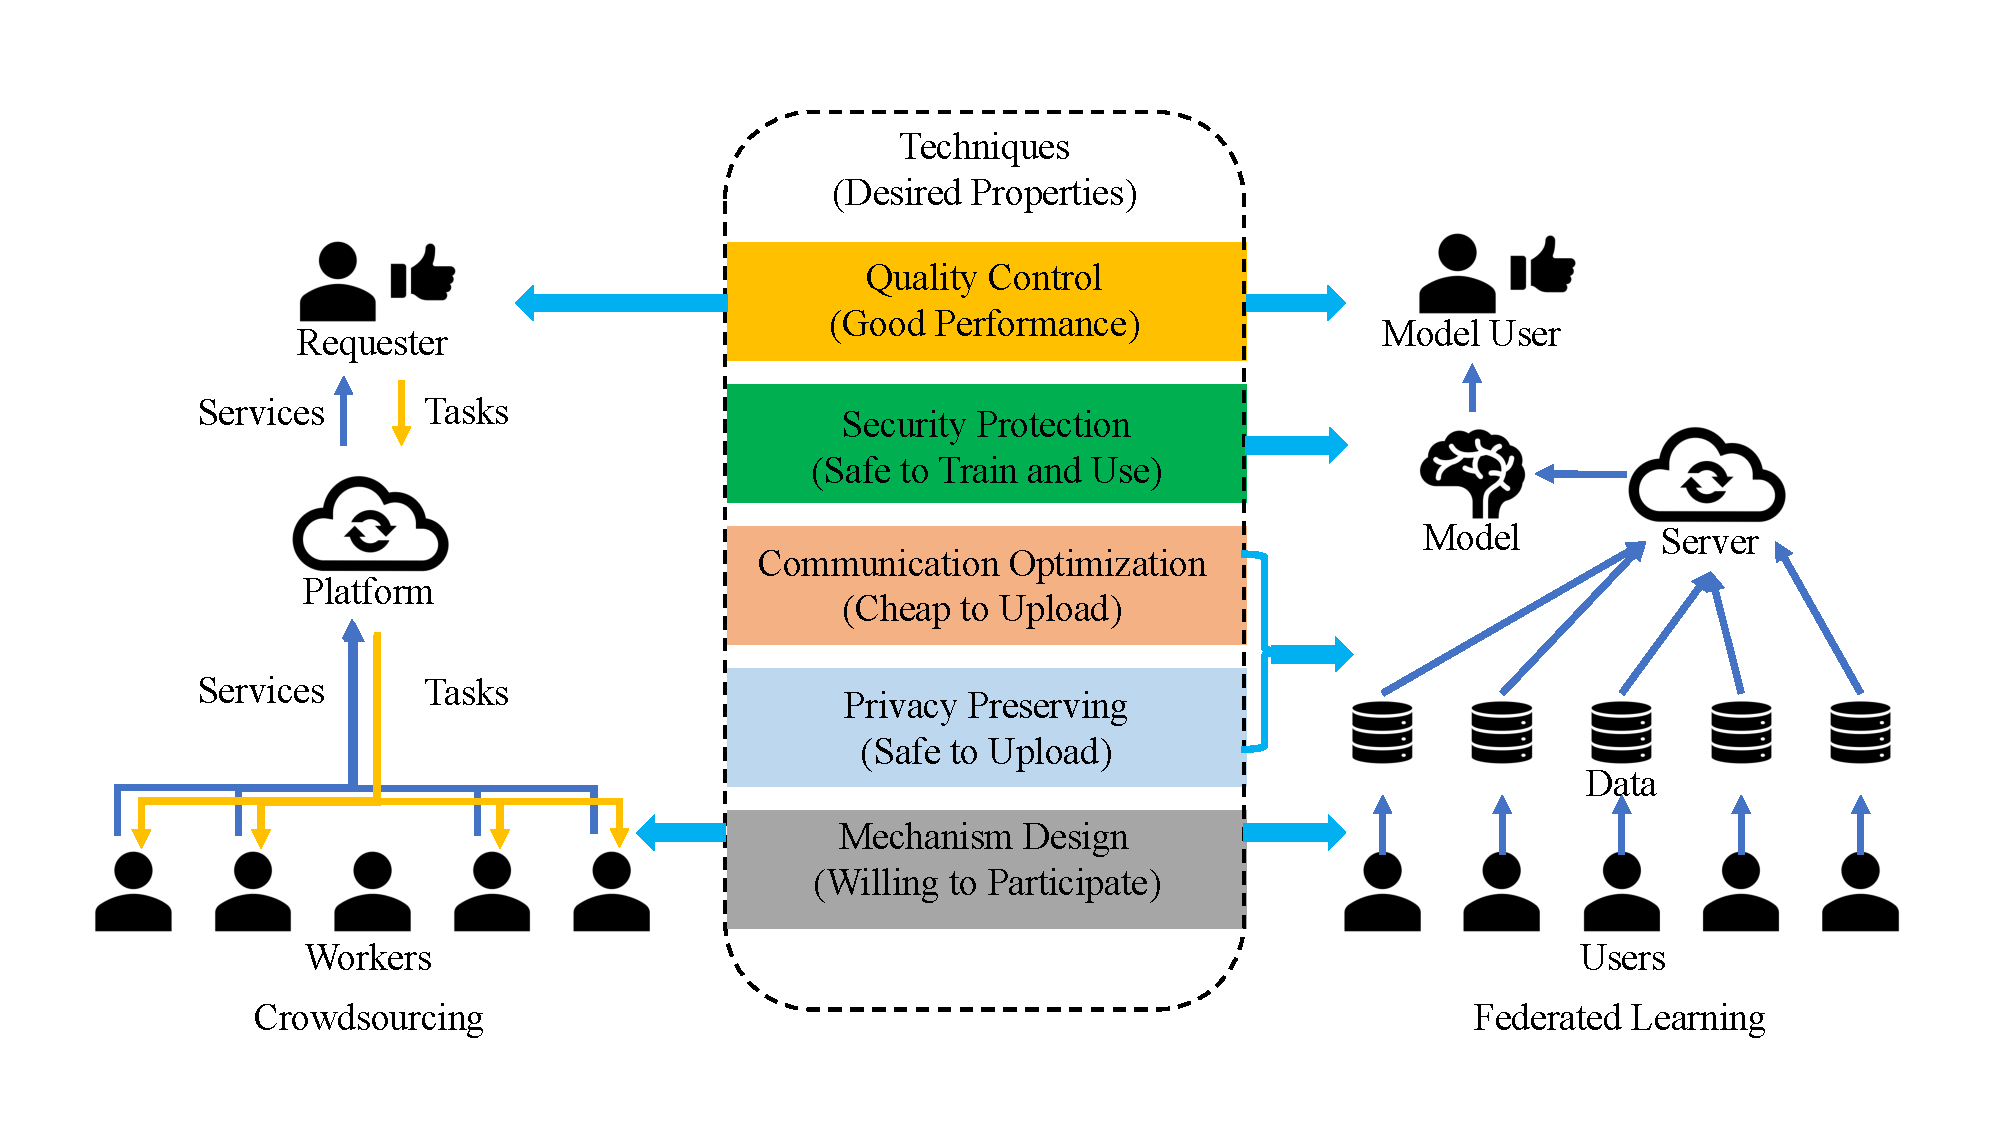
\includegraphics[width=\textwidth]{figs/comparison.png}
%     \caption{Caption}
%     \label{fig:enter-label}
% \end{figure}


\stitle{Why-DP-Provenance}, also known as output-provenance, refers to the additional information that helps data analysts understand the reasoning behind a DP system's output. It focuses on the interaction between the system's results and the analyst's needs.
Why-DP-provenance aims to answer questions like, \emph{why is a specific privacy budget chosen for the analyst's query, how does the level of noise in the answer achieve the desired accuracy, why is a noisy answer still considered useful, and what factors lead to a query rejection?}
Benefits of enforcing fine-grained why-DP-provenance include:
\begin{itemize}
    \item \emph{Explainability and Interpretability}: Why-DP-provenance details query answers' usefulness and confidence intervals, which allows analysts to understand the trade-offs between privacy guarantees and accuracy.
    \item \emph{Tighter Privacy Composition:} Why-DP-provenance facilitates a more accurate understanding of how different queries impact the overall privacy budget. \item \emph{Optimal Privacy-Accuracy Trade-Offs:} Why-DP-provenance empowers analysts to make informed decisions about the balance between privacy and the usefulness of results. 
\end{itemize}
Techniques for why-DP-provenance device approaches for accuracy-first query specification, error specification, fine-grained budget specification, and others.
Unlike the why-provenance in databases that focuses on ``why'' something happened or exists, the why-DP-provenance answers ``why'' a specific level of parameters in a DP algorithm is chosen and its impact on results within a DP system.





\stitle{How-DP-Provenance}, also known as process-provenance, focuses on capturing details about the specific privacy mechanisms employed within a DP system. This information becomes crucial for answering complex queries privately, building complex DP mechanisms, or selecting the optimal/best DP mechanisms for a query workload.
How-DP-provenance solves the following questions: \emph{How is the noise for a private query calculated based on a series of transformations of data? What structural properties of a query can be used for a tighter privacy bound? Can we reuse the noise calibrated to historical queries for answering new queries to save the privacy budget?}
Fine-grained how-DP-provenance tracking enables: 
\begin{itemize}
    \item \emph{Efficient Privacy Analysis:} How-DP-provenance tracks the series of modularized transformations or the query structural properties for complex queries to make sensitivity analysis more efficient.
    \item \emph{Better Utility for Query Workloads:} How-DP-provenance reuses noise from historical query answers or injects correlated noise to a batch of queries to increase the overall utility for the workload.
    \item \emph{Effective Budget Allocation:} How-DP-provenance facilitates the budget allocation across multiple data analysts so that the privacy loss is tightened when analysts collude.
\end{itemize}
Techniques that support fine-grained how-DP-provenance include transformation tracking and noise tracking.
Different from the how-provenance in databases that generates a derivability relationship between output and input tuples, the how-DP-provenance answers ``how'' a better DP mechanism could be designed or modularized for answering queries.



\stitle{Where-DP-Provenance}, also known as input-provenance, accounts for which (part of) private input data is used for a DP mechanism.
The complex data type can involve multiple database tables, and queries over different tables can result in different DP guarantees --- tracking which tables are used for what queries becomes essential for multi-relational DP systems.
Furthermore, even with a single table, different queries or mechanisms may be interested in different parts of the table --- accounting privacy loss at the table-level can waste more privacy budgets.
Third, data may be merged at different timestamps or belong to different users.
Thereby, where-DP-provenance tracks privacy loss for data by answering questions of \emph{what part of the private data is used to answer a particular query, what (group of) users are associated with the data.}
With where-DP-provenance, the system gains:
\begin{itemize}
    \item \emph{Flexibility with Multi-Resolution Privacy}: Where-DP-provenance allows data curators to specify policies with different resolutions of privacy guarantees.
    \item \emph{Continuously Running System}: Where-DP-provenance enables the replacement of retired data with new data so that the system can continuously execute.
\end{itemize}
While the where-provenance in databases pinpoints the exact places that an output tuple is copied from, the where-DP-provenance answers ``where'' incurs a privacy loss in the private input w.r.t queries.





Next, we will describe the DP techniques that fit into the framework of each why, how, and where-DP-provenance and the different granularities of these techniques.


\subsubsection{Techniques for Why-DP-Provenance}


\stitle{Query Specification.}
Two types of DP query specification exist: \emph{privacy-first} and \emph{accuracy-first}.
Most (traditional) DP building blocks or systems are \emph{privacy-first}, meaning that they require the data analysts to specify a privacy budget for their queries or tasks to run.
This privacy budget will be deducted from the global privacy budget if the tasks are executed and the noisy answers are returned to the analysts.
While this approach is easy to analyze and has many optimal and off-the-shelf mechanisms developed over the years, it may limit the usability of a DP system: the data analysts care about the quality of the query answers, but may not have sufficient expertise to understand the DP mechanisms and the relationship between privacy and the error rate according to the chosen mechanism.
Since a DP system cannot release the true query answer, a single noisy output cannot explain how well the black-box mechanism works to privacy novice analysts.
In addition, the released answers (or consumed budget) can not be reversed—discarding unsatisfactory query answers simply wastes the global privacy budget.


Another approach for query specification is \textit{accuracy-first}~\cite{ge2019apex,Ghayyur2022mide,dprovdb,WhitehouseRWR22brownian,xiao2021optimizing,ligett2017accuracy,mazmudar2022cache,pioneer}, that allows the data analysts to superimpose an accuracy requirement in the query specification, and the system can translate the accuracy requirements into privacy budget and automatically choose the optimal mechanism to answer this query.
This approach aims to close the discrepancy between privacy-oriented DP mechanisms and the needs of data analysts for understanding noisy outputs, but many open problems remain in understanding data-dependent accuracy translation.
Recent work like DPella~\cite{lobo2020programming} and DProvDB~\cite{dprovdb} support both the privacy- and accuracy-oriented modes.





\stitle{Error Specification.} 
A line of work, including DPComp~\cite{hay2016exploring}, Overlook~\cite{thaker2020overlook}, PSI~\cite{gaboardi2016psi}, Bittner et al.~\cite{bittner2020understanding}, DPP~\cite{john2021decision}, ViP~\cite{NanayakkaraB0HR22visualizing}, and DPXPlain~\cite{TaoGMR22DPXPlain}, aims to provide interfaces for explaining the noisy output to the data analyst or visualizing an optimal privacy-utility trade-off due to the mechanism to help the analysts make informed choices.
These tools explore a DP confidence interval of the noisy answer~\cite{covington2021unbiased,du2020differentially,cohen2023optimal,drechsler2022nonparametric,NanayakkaraB0HR22visualizing,SunDY23CI} or other statistical metrics on measuring accuracy of the answer as functions of the selected privacy budget~\cite{thaker2020overlook,john2021decision}.
ViP~\cite{NanayakkaraB0HR22visualizing} associates the query output with a differentially private randomization interval, indicating the noise bounds of the query result with high confidence.
This randomization bound could be either post-processed from a noisy answer if the mechanism is data-independent or computed with a small portion of additional privacy budget from data-dependent mechanisms~\cite{covington2021unbiased,du2020differentially,cohen2023optimal,drechsler2022nonparametric}.
DPXPlain~\cite{TaoGMR22DPXPlain}, on the other hand, start to explore methods of providing additional explanation of aggregation query results, on which whether an unexpected answer is due to the data itself or the randomness introduced by DP.
 
\stitle{Budget Specification.} 
The composition of privacy loss through a series of queries can be classified into two levels, based on whether different analysts are distinguished.
The coarser level of query composition is to regard all data analysts as a unified entity, and the system sequential composition to account for privacy loss during the execution of the queries.
This method is easy to implement, well-suited to different types of (complex) queries, and can explain whether a query is rejected—the privacy budget or the translated privacy budget exceeds the remaining global privacy budget.
Sequential composition can also be replaced by a privacy odometer~\cite{RogersVRU16odometer,lecuyer2021odometer} or adaptive composition~\cite{whitehouse2023fully,winograd2017framework,kairouz15} that gives tighter privacy bound over the queries that are adaptively asked, but they are restricted to simple queries.
More fine-grained query composition is to track the privacy loss as per data analysts and per queries they ask~\cite{dprovdb}.
This approach can not only answer more specific questions on \textit{why this particular analyst's query is rejected} but also achieve fairness among multiple data analysts when they are assigned different trust/privilege levels.
However, fine-grained tracking requires recording more metadata proportional to the number of data analysts in the system.


\stitle{Other Techniques for Why-DP-Provenance: Automated DP Proof Generation.}
Besides explaining noisy output to the data analysts, another line of work investigates the logical representation and execution of a differentially private mechanism/system.
They check and verify the privacy properties of a DP program implementation by either generating automated proofs for DP~\cite{wang2021dpgen,abuah2021dduo,wang2020checkdp,wang2019proving,zhang2017lightdp,near2019duet,solo22} or detecting counterexamples that violate DP guarantees~\cite{ding2018detecting,bichsel2018dp,bichsel2021dp,barthe2020deciding} through annotated type systems and static/dynamic analysis of the program execution.



\subsubsection{Techniques for How-DP-Provenance}

\stitle{Transformation Tracking.}
Complex database queries often consist of a series of transformations over the private data, e.g., selection, projection, group-by, join, union, and aggregation. 
In order to calibrate noise to the query answers, the system needs to analyze the sensitivity of the query.
We categorize the approaches to estimate the sensitivity of a query into three levels, from coarse-grained to fine-grained: tracking sensitivity directly, tracking transformation stability, and tracking query structures.

\noindent
\emph{Tracking Sensitivity (Directly).}
The coarsest level of how-DP-provenance is to directly compute an upper bound of the query sensitivity.
For simple queries, the sensitivities are well understood and can be computed easily.
However, for complex queries, without making clever use of the properties of the query, the sensitivity could be overestimated or cumbersome to compute.

\noindent
\emph{Tracking Transformation Stability.}
Existing systems like PINQ~\cite{mcsherry2009pinq} and wPINQ~\cite{ProserpioGM14wpinq} keep track of the \textit{transformation stability} to calculate the amount of noise needed for the queries.
For a transformation $T: \mc{D} \rightarrow \mc{D}$, it is $c$-stable if $\forall$ two input databases $D, D' \in \mc{D}$, we have $| T(D) \triangle T(D') | \leq c \times |D \triangle D'|$, where $\triangle$ denotes the symmetric difference between two databases, i.e., $D \triangle D' = (D \backslash D') \cup (D' \backslash D)$.
For example, common SQL transformations selection, projection, and counting queries have stability of 1, and group-by has a stability of 2.
It has been shown that for a $\epsilon$-differentially private mechanism $\mc{M}$ and a $c$-stable transformation series $T$, the composition $\mc{M} \circ T$ will be $(c \cdot \epsilon)$-differentially private.


\noindent
\emph{Tracking Query Structures.}
Keeping the transformation stability metadata makes it easy to analyze the privacy loss for a series of linear transformations before histogram queries, but may not be sufficient for highly sensitive queries like aggregation and join.
The query sensitivity for aggregations could be as large as the size of the domain product (e.g., sum over selected attributes).
The approach to handling aggregation queries is to truncate the attribute domain~\cite{johnson2020chorus,FangD022shifted,dong2023universal} and/or perform aggregations on disjoint subsamples~\cite{nissim2007smooth,mohan2012gupt,Smith11sample_aggregate,johnson2020chorus}, which requires the system to keep track of the truncation information per query and per attribute and the information about how the truncation transfers over queries.
Chorus~\cite{johnson2020chorus} enables a query rewriting and annotation technique, which could be seen as using \textit{how-DP-provenance}, to automatically trace and analyze the query stability and truncated domain when processing aggregation queries.
Similarly, the sensitivity of join queries can be even unbounded — changing one tuple in an input table can cause unbounded changes in the join output since this tuple can match an arbitrary number of tuples in another input table.
DP mechanisms for answering join queries clip the maximum number of tuples that a tuple can match in a join~\cite{kotsogiannis2019privatesql}, or add data-dependent noises~\cite{nissim2007smooth,johnson2018towards,dong2021residual,dong2021nearly}, or a mixture of both~\cite{dong2022r2t}.
Indeed, the recent residual sensitivity mechanism~\cite{dong2021residual} analyzes the multi-way join topology metadata and traces a smooth upper bound of local sensitivity across this join topology to \textit{efficiently} calculate a \textit{tighter} noise.


\stitle{Noise Tracking.}
While the basic DP system does not track the noise added to each query answer (i.e., queries are regarded as independent), a number of recent work~\cite{dprovdb,mazmudar2022cache,xiao2022answering,li2014data,hardt2010multiplicative,KostopoulouTCGL23turbo} inject correlated noise to the answers.
They optimize the accuracy of the query results by batching the query workload and adding correlated noise with the \emph{workload of one single data analyst}~\cite{xiao2021optimizing,li2014data,dong23composition}, or, in a more fine-grained way, maintaining a stateful cache of the historical query answers~\cite{mazmudar2022cache,KostopoulouTCGL23turbo,kotsogiannis2019privatesql} so that answers to the new queries can reuse the cached noises.
The DP caches are extended from answering one data analyst's queries to mitigating privacy loss across multiple data analysts~\cite{dprovdb,DworkNV12power_of_state,nicolas2023cohere,HsuRU13equilibrium} or tight adaptive composition~\cite{vadhan2021concurrent,vadhan2023concurrent} across analysts when multiple analysts ask the same or similar queries.
Other multi-analyst systems~\cite{xiao2021optimizing,xiao2022answering,knopf2021framework,pujol2021budget,pujol2022multi} tracks per-analyst privacy \cite{xiao2021optimizing} or accuracy \cite{knopf2021framework} constraints to optimize the privacy-accuracy trade-off or fairly answer queries among analysts \cite{pujol2021budget,pujol2022multi}.
Among all the different settings in multi-analyst DP, additional fine-grained requirements or privacy guarantees regarding different analysts' queries are recorded for the DP mechanism designs, which is in line with how-DP-provenance.



\subsubsection{Techniques for Where-DP-Provenance}

\stitle{Privacy Resolutions.} 
Depending on the data model and the intended privacy goals to deliver, a DP system can achieve the notion of \textit{event-level DP}, \textit{user-level DP}, \emph{multi-resolution DP} (defined as per policies)~\cite{he2014blowfish,kotsogiannis2019privatesql} and other extended notions of DP, e.g., personalized user-level DP~\cite{jorgensen2015personalized}.
Event-level DP assumes that in the private input data, each individual contributes only one record, while it is a special case of user-level DP, which allows each individual to make multiple contributions and reasons about privacy at the user level.
In particular, the neighboring database definition is different in the two settings, which changes the way sensitivity is analyzed.
Other DP notions, such as Pufferfish privacy~\cite{kifer2014pufferfish}, Blowfish privacy~\cite{he2014blowfish}, multi-resolution privacy~\cite{kotsogiannis2019privatesql}, per-attribute DP\cite{Ghazi0M023per_attr_DP}, Metric DP~\cite{chatzikokolakis2013broadening}, geo-indistinguishability~\cite{yu2022thwarting}, etc., relax and extend DP to more general settings for example with correlations.


\stitle{Privacy Accounting.} 
Accounting for privacy loss over the input data is challenging.
The basic DP system performs the privacy composition at the table level.
However, it is unlikely that every query touches the entire table.
Accounting privacy at the table level would waste privacy budgets for the part of data that is not used for computations.
More fine-grained privacy accounting considers splitting databases into disjoint blocks and sub-tables, and only the block that is used for answering a query will be deducted for privacy consumption.
This approach is called parallel composition or block composition~\cite{mcsherry2009pinq,LecuyerSVG019sage}.
This has also been extended in recent work~\cite{nicolas2023cohere} that a finer-grained user-level partitioning is available at the column level so that the wasted privacy budget can be minimized.
Other than privacy accounting for different parts of the data, the input data can arrive at different timestamps.
Based on the DP models used, existing work proposes mechanisms for sliding windows~\cite{kellaris2014differentially}, the entire streams~\cite{DworkNPRY10panprivate,dong2024continual,DongLY23continual} or with historical data~\cite{growingdb18}.




\begin{table}
\caption{Taxonomy of Privacy Provenance and Evaluations of Implemented DP Systems. \cmark=with, \xmark=without, \Circle=Coarse-Grained, \LEFTcircle=Moderate-Grained, \CIRCLE=Fine-Grained. Shaded rows indicate systems surveyed in case studies. 
}
\scriptsize	
%\begin{adjustbox}{width=1\textwidth}
    \begin{tabular}{@{}llclllll@{}}
        \toprule
        \multirow{2}{*}{Systems} & \multicolumn{3}{c}{Why-DP-Provenance}                  & \multicolumn{2}{c}{How-DP-Provenance}    & \multicolumn{2}{c}{Where-DP-Provenance} \\ \cmidrule(lr){2-4} \cmidrule(lr){5-6} \cmidrule(l){7-8} & Query Spec     & Err Spec & Budget Spec & Transformation  & Noise (Trackings) & Priv Resolutions    & Priv Accountant   \\ \hline
Basic                    & Privacy-First  & \xmark   & \Circle ~Per Query     & \Circle ~Sens Only          & \xmark ~No            & \Circle ~Event-DP    & \Circle ~Table Level          \\
PINQ~(\citeyear{mcsherry2009pinq})                     & Privacy-First  & \xmark   & \Circle ~Per Query     & \LEFTcircle ~Sens+Stability & \xmark ~No            & \Circle ~Event-DP    & \LEFTcircle ~Sub-Table Level  \\
ProPer~(\citeyear{ebadi2015differential})                   & Privacy-First  & \xmark  & \Circle ~Per Query     & \LEFTcircle ~Sens+Stability & \xmark ~No            & \CIRCLE ~User-DP\textsuperscript{\textdagger}     & \LEFTcircle ~Sub-Table Level \\
PSI$\Psi$~(\citeyear{gaboardi2016psi}) &Privacy-First & \LEFTcircle & \LEFTcircle ~Per Query\textsuperscript{*} &\Circle ~Sens Only & \xmark ~No  & \Circle ~Event-DP & \Circle ~Table Level   \\
$\epsilon${\sc ktelo}~(\citeyear{zhang2018ektelo})   &Privacy-First & \xmark&\Circle ~Per Query& \LEFTcircle ~Sens+Stability & \LEFTcircle ~Workload & \Circle ~Event-DP &\LEFTcircle ~Sub-Table Level \\  
\rowcolor{Gray}                                 
APEx~(\citeyear{ge2019apex})                     & Accuracy-First & \Circle   & \Circle ~Per Query     & \Circle ~Sens Only          & \LEFTcircle ~Workload & \Circle ~Event-DP    & \Circle ~Table Level          \\
PrivateSQL~(\citeyear{kotsogiannis2019privatesql}) & Privacy-First & \xmark & \Circle ~Per Query & \Circle ~Sens Only & \CIRCLE ~Caching & \CIRCLE ~Policy-DP& \Circle ~Table Level\\
\rowcolor{Gray}                                   Sage~(\citeyear{LecuyerSVG019sage})                     & Privacy-First  & \xmark   & \Circle ~Per Query     & \Circle ~Sens Only          & \xmark ~No            & \Circle ~Event-DP    & \LEFTcircle ~Sub-Table Level  \\
Chorus~(\citeyear{johnson2020chorus})                   & Privacy-First  & \xmark   & \Circle ~Per Query     & \CIRCLE ~Query Struct    & \xmark ~No            & \Circle ~Event-DP    & \Circle ~Table Level        \\
CacheDP~(\citeyear{mazmudar2022cache})&Accuracy-First & \Circle&\Circle ~Per Query & \Circle ~Sens Only & \CIRCLE ~Caching & \Circle ~Event-DP & \Circle ~Table Level \\
ViP~(\citeyear{NanayakkaraB0HR22visualizing}) & Privacy-First & \CIRCLE & \LEFTcircle ~Per Query\textsuperscript{*}  & \Circle ~Sens Only  & \xmark ~No & \Circle ~Event-DP & \Circle ~Table Level\\
\rowcolor{Gray}                                 
DProvDB~(\citeyear{dprovdb})                  & Both & \Circle   & \CIRCLE ~Query+Analyst & \LEFTcircle ~Sens+Stability & \CIRCLE ~Caching      & \Circle ~Event-DP    & \Circle ~Table Level          \\
\rowcolor{Gray}                                   Cohere~(\citeyear{nicolas2023cohere})                   & Privacy-First  & \xmark   & \CIRCLE ~Query+Analyst & \Circle ~Sens Only          & \LEFTcircle ~Workload & \LEFTcircle ~User-DP & \CIRCLE ~Column Level         \\


\bottomrule
                                 
        \end{tabular}
%\end{adjustbox}
\flushleft{
\rule{0in}{0em}{ \footnotesize \textsuperscript{\textdagger} ProPer achieves user-level DP with personalized privacy guarantees.}\\
\rule{0in}{0em}{ \footnotesize \textsuperscript{*} ViP and PSI$\Psi$ both support an interface to help analysts split privacy budget across multiple queries. ViP supports more types of error specifications (confidence intervals, quantiles, etc.).}
}
\label{tab:taxonomy}
\end{table}

% \begin{figure}
%     \centering
%     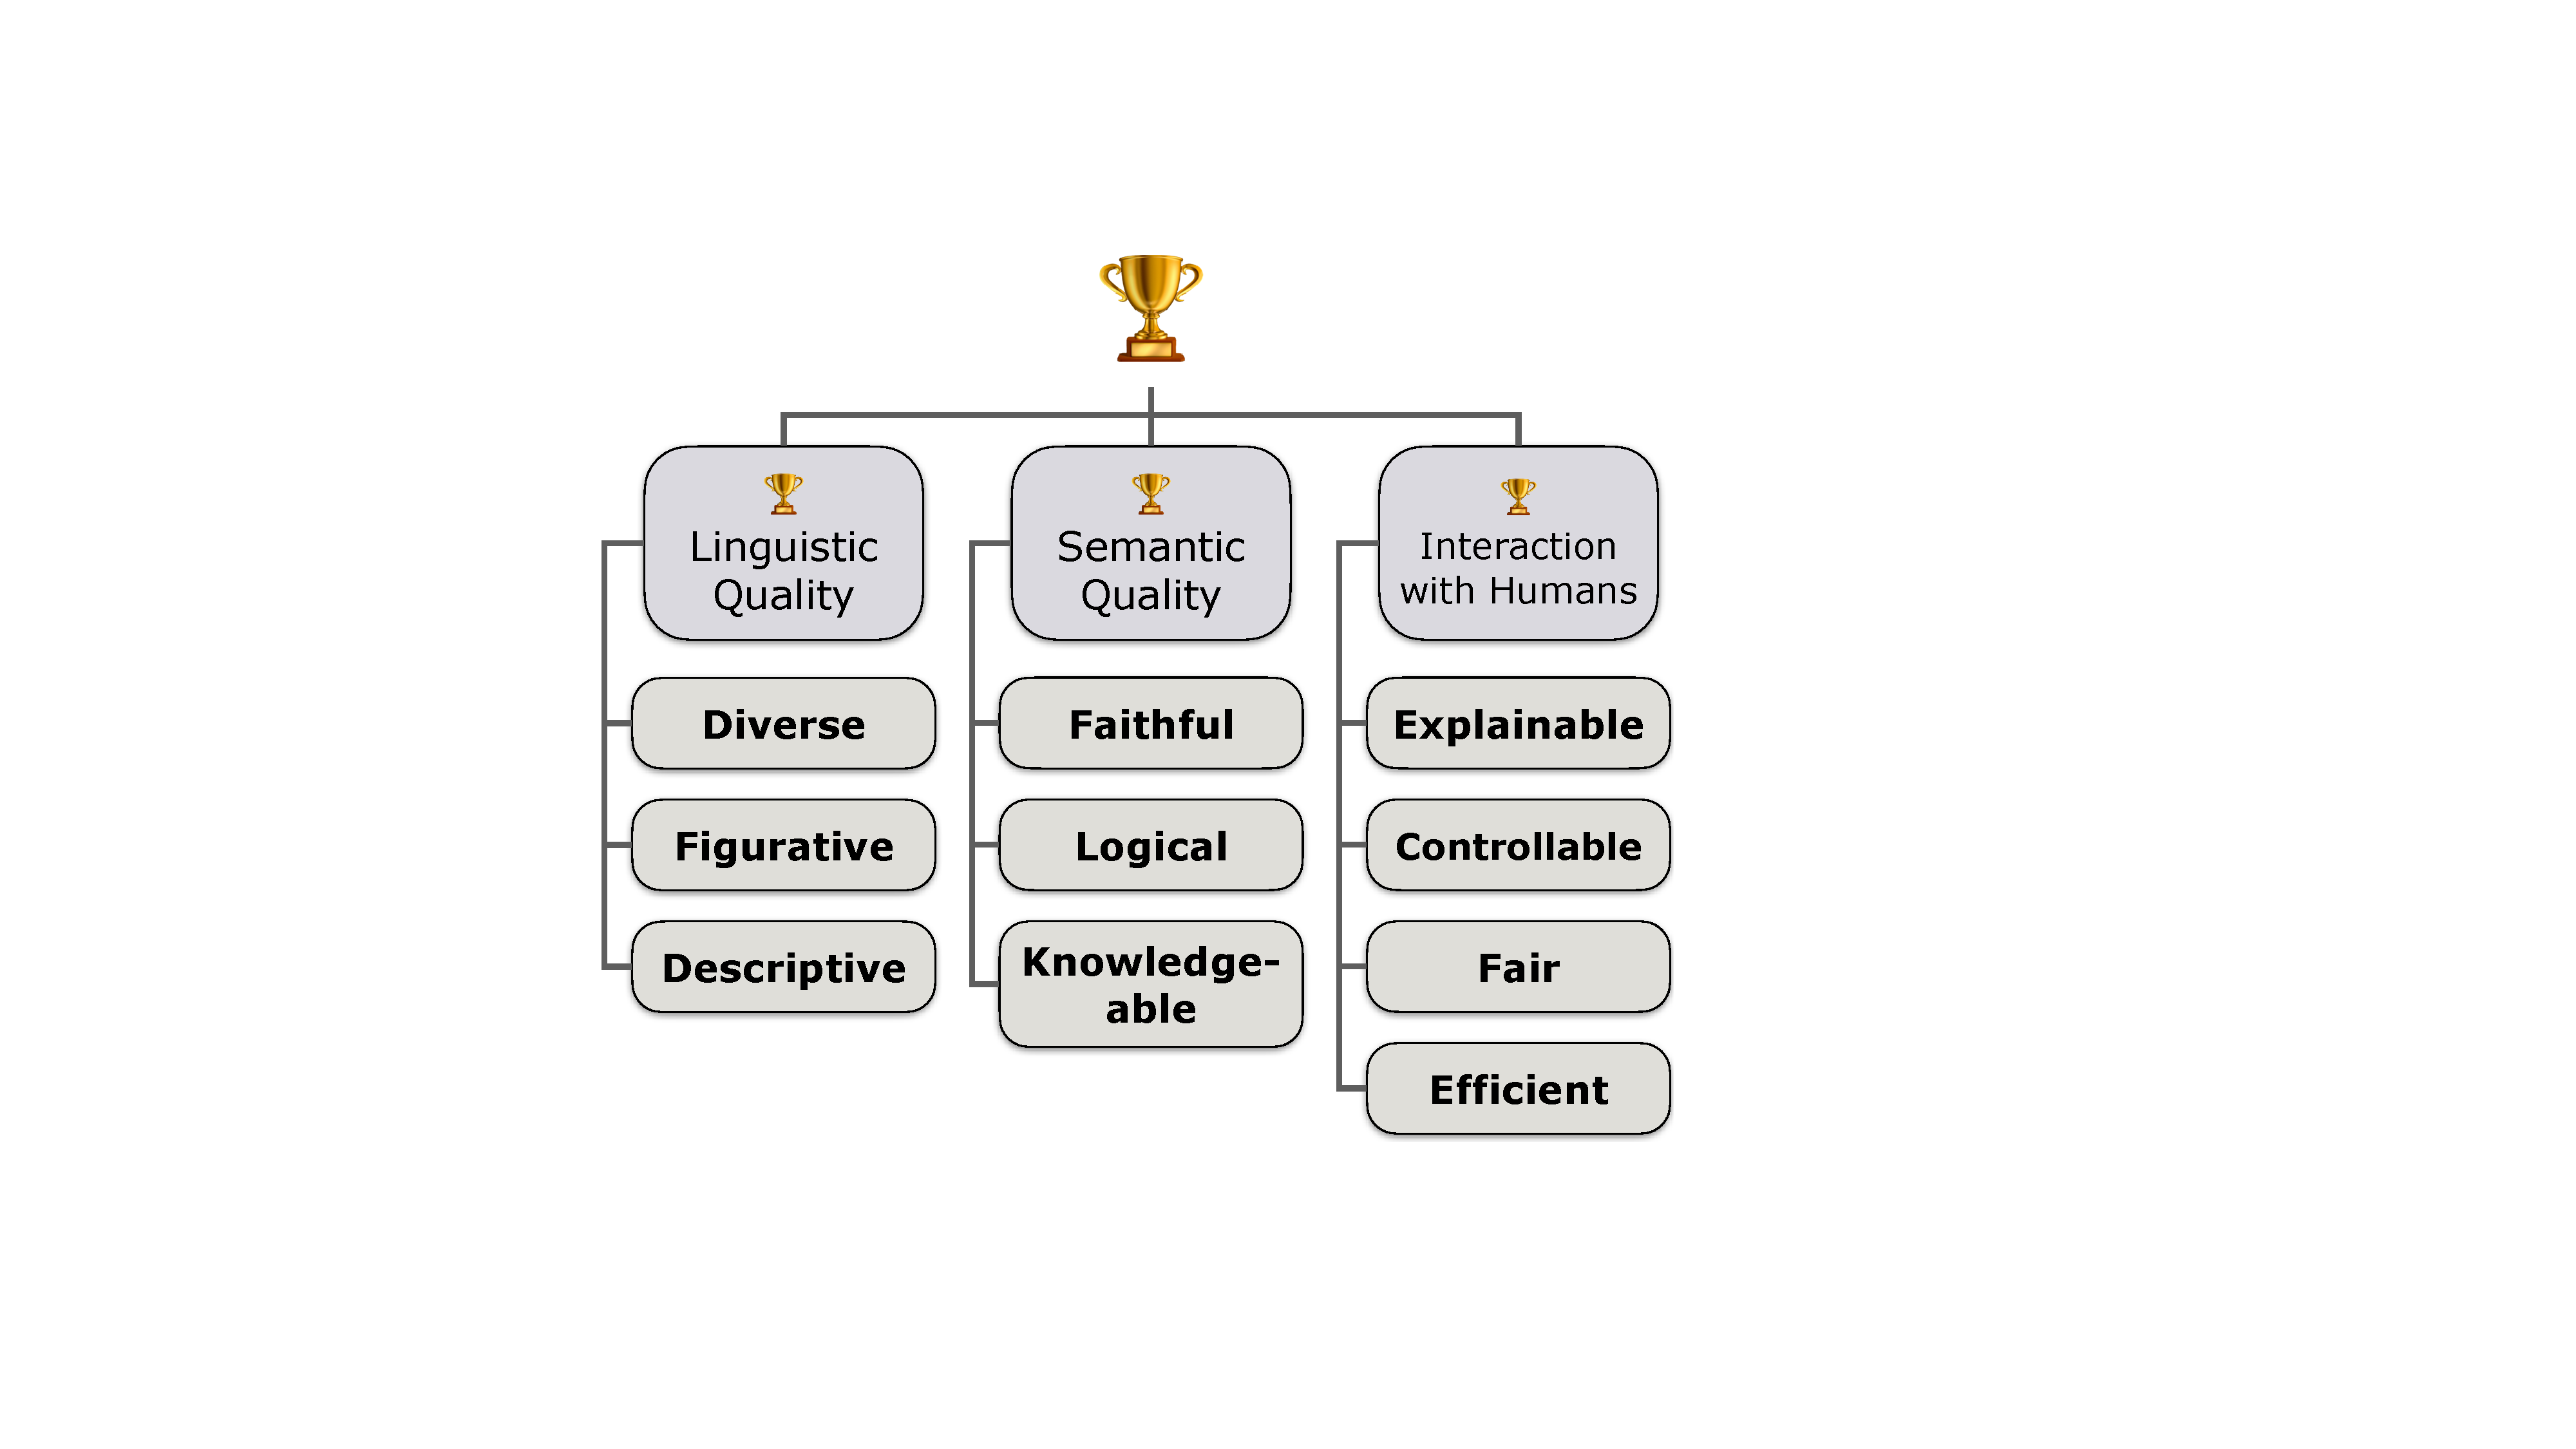
\includegraphics[width=\textwidth]{figs/taxonomy.png}
%     \caption{}
%     \label{fig:enter-label}
% \end{figure}



\bigskip

\noindent
Table~\ref{tab:taxonomy} summarizes the techniques and the granularities of the provenances used in some existing DP systems for DP with trusted data curators (i.e., in the central setting). We discuss other cases that enforce local DP or other models of DP in Section 5.

\section{Case Studies on Systems with Fine-Grained Privacy Provenance}

This section dives into several representative DP systems that utilize fine-grained why-, how-, and where-provenance techniques via case studies. Each case study overviews the related systems, summarizes their provenance techniques, and discusses their strengths and weaknesses.


\subsection{Case Study: APEx for Accuracy-Aware DP Data Exploration}

APEx prioritizes accuracy in query specification through why-DP-provenance techniques. Additionally, it employs noise tracking for processing exploration workloads, leveraging how-DP-provenance. These features enhance the usability of the basic DP system.

\subsubsection{Problem and Technical Brief}
APEx is among the first systems to empower data analysts, even those without prior DP expertise, to easily specify private queries. It achieves this by allowing analysts to focus on their desired outcome, the answer's accuracy, rather than needing to grapple with complex privacy budgets. This ability to specify accuracy expectations exemplifies \underline{why-DP-provenance} in action, as it provides valuable information about the usefulness and confidence intervals of query results. This feature ultimately enhances the user experience with DP systems. To achieve this user-centric approach, APEx made several vital contributions: 
\begin{itemize}
    \item A New Language for DP Queries: APEx designed a new, SQL-like query language tailored for DP tasks. This language simplifies query specification for analysts.
    \item Accuracy-Privacy Translation Framework: APEx developed a framework that automatically translates an analyst's desired accuracy level into an optimal DP mechanism. This framework eliminates the need for analysts to choose a mechanism themselves. APEx also compiled a comprehensive library of the latest DP mechanisms, ensuring the framework has the best one to achieve the desired accuracy-privacy trade-off. 
\end{itemize}
In addition to these why-provenance advancements, APEx also introduced a novel data-dependent DP mechanism that leverages \underline{how-DP-provenance}. This mechanism tracks the noise added during query processing to minimize privacy costs while still meeting the specified accuracy requirements. We will delve deeper into each of these contributions in the following sections.


\stitle{Query Language with Accuracy Measures.}
APEx aims to support SQL-like declarative query languages with accuracy specifications.
The syntax of the query language is defined in the following format.
\begin{center}
\begin{tabular}{c}
\begin{lstlisting}[mathescape=true]
BIN $D$ ON $f(\cdot)$ WHERE $W=\{\phi_1,\ldots,\phi_L\}$
[HAVING $f(\cdot)>c$]
[ORDER BY $f(\cdot)$ LIMIT $k$]
ERROR $\alpha$ CONFIDENCE $1-\beta$;
\end{lstlisting}
\end{tabular}
\end{center}

The meaning of this query syntax is to map a database $D$ into bins of rows $\{b_1,\ldots,b_L\}$ based on a workload of predicates $W=\{\phi_1,\ldots,\phi_L\}$, where each bin $b_i$ contains rows that satisfy the predicate $\phi_i$. Then it applies the aggregation function $f(\dot)$ (e.g., count and sum) over each bin $b_i$.
The two lines in the brackets are optional. A \textit{workload counting query} (WCQ) is simply the query when $f()$ is a counting function that returns the bin size without the two optional lines. A similar query with the HAVING clause is an \textit{iceberg counting query} (ICQ) that returns a list of bin identifiers $b_i$ for which $f(b_i) > c$, and a query with the ORDER BY ... LIMIT clause is called the \textit{top-k counting query} (TCQ) that returns the $k$ bins that have the largest values for $f(b_i)$.

For a query with a numerical output like WCQ, there are multiple accuracy semantics considered by the literature, such as mean square error (MSE)~\cite{XiaoBHG11relativeerror}, relative error~\cite{XiaoBHG11relativeerror}, and $(\alpha,\beta)$-accuracy~\cite{dwork2014algorithmic}. APEx considers $(\alpha,\beta)$-accuracy for WCQ and extends it to non-numerical queries like ICQ and TCQ. In particular, we say a mechanism $M$ satisfies $(\alpha,\beta)$-WCQ accuracy, if with a high probability $1-\beta$, for each predicate $\phi\in W$,
the absolute difference between its noisy answer returned by $M$ and its true answer is bounded by $\alpha$, i.e., $$\Pr[\max_{\phi\in W}|M_{\phi}(D)-c_{\phi}(D)|\leq \alpha]\geq 1-\beta.$$ For a non-numerical query like ICQ, APEx has two parts for its accuracy requirement: 
$$\Pr[|\{\phi \in M(D) ~|~ c_{\phi}(D) < c-\alpha\}|>0] \leq \beta$$
$$\Pr[|\{\phi \in (W-M(D)) ~|~ c_{\phi}(D) > c+\alpha\}|>0] \leq \beta$$ simultaneously. This first part corresponds to the type I error that wrongly labels predicates with a true count less than $c$ as $>c$. The second part is for the type II error that labels the predicates with a true count greater than $c$ as $<c$.
The accuracy definition is satisfied if, with a high probability of $1-\beta$, all predicates with true counts greater than $ c+\alpha$ or less than $ c-\alpha$ are correctly labelled.
APEx extends the same logic to the accuracy requirement for TCQ in a similar flavor.
Note that both $(\alpha,\beta)$-ICQ accuracy and $(\alpha,\beta)$-TCQ accuracy definitions consider \textit{symmetric} errors. 
Definitions and mechanisms that extend to \textit{asymmetric} errors are discussed and proposed in the MIDE system for private decision-making~\cite {Ghayyur2022mide}.


\stitle{Accuracy-Privacy Translation Framework.} 
For each query and its accuracy specification, APEx automatically finds the best mechanism that satisfies the accuracy specification of the query with the least privacy budget. First, APEx prepares all the existing DP mechanisms and executes them in two phases: (i) privacy cost estimation, which simulates how much privacy budget would be needed if the mechanism were used, and (ii) running the algorithm, which actually runs the mechanism and returns the answer to the data analysts. Second, APEx stores all the relevant state-of-the-art DP mechanisms for each query type since the best one depends on the query and the data. For example, for WCQ, APEx provides two data-independent translation mechanisms. The first data-independent mechanism is the baseline \textit{Laplace mechanism}, which analyzes the error bounds of Laplace noise and obtains directly a closed-form expression of bounds on the translated privacy budgets.
The second mechanism, \textit{strategy-based mechanism}, 
uses the matrix mechanism~\cite{li2014data,LiMHMR15} to analyze the overlapping parts of the workload $W$ and reuse the noisy intermediate results for the overlapping part to translate the same accuracy target into, in many cases, a tighter bound on privacy budget. The strategy-based mechanism is also data-independent and can be generalized to all the query types.

\stitle{Data Dependent Accuracy-Privacy Translation.} APEx considers a data-dependent accuracy-privacy translation mechanism for ICQ, an example of how-DP-provenance.
An ICQ involves comparing the bin sizes with the threshold value $c$. For example, the data-dependent Laplace mechanism adds noise to the true bin sizes and compares the noisy bin sizes with the threshold. For example, given an accuracy target $\alpha=10, \beta=0.00001$, APEx will translate this into budget $\frac{\ln{(1/2\beta)}}{\alpha} = 0.85$ for the Laplace mechanism. However, if the bin sizes are far away from the threshold, let's say $c_{\phi}(D)=1000$ and the threshold is $c=100$ where the difference is 90 times $\alpha$, then it may be sufficient only to use $\frac{0.85}{90} \approx 0.01$ privacy budget. As APEx does not know the distance between the true bin sizes and the threshold, it proposes a \textit{multi-poking mechanism} that starts with a small privacy budget and tests multiple times with increasing privacy budgets until it can determine the noisy answer would satisfy the accuracy target confidently. 
Rather than drawing independent Laplace noise in each iteration, this multi-poking mechanism stores the privacy budgets and the noise used in previous ``pokings'' and samples correlated noise each time~\cite{koufogiannis2015gradual}. This correlated noise allows the overall privacy loss to be bounded by the privacy budget of the last poking instead of the sum of the privacy budgets over all the poking steps.

\subsubsection{Improvements and Limitations}
APEx offers several advantages that make it easier to conduct private data analysis:
1) \textit{usability improvement via why-DP-provenance}, where APEx empowers data analysts, even those without prior privacy expertise, to achieve high accuracy in tasks like entity resolution, as shown in its user studies; 2) \emph{privacy improvement via how-DP provenance}, where the new multi-poking mechanism significantly reduces the privacy budget needed for specific workloads (4 out of 8 ICQ workloads in studies) compared to traditional approaches.
While APEx offers significant benefits, it is essential to acknowledge some limitations: 1) \textit{compatibility with accuracy bounds}, for not all data privacy algorithms have clearly defined accuracy limitations, which restricts APEx's ability to incorporate them into its framework; 2) \textit{runtime overheads}, for 
APEx requires running all the relevant mechanisms and storing/tracing the correlated noise calibration in the multi-poking mechanism, though they are relatively small and are only needed at runtime.





\subsection{Case Study: DProvDB for Multi-Analyst DP}
Unlike prior systems, DProvDB enforces privacy constraints, not only on the queries and the input data but also on each analyst. This design aims to achieve a fair distribution of privacy budget among data analysts and a tight privacy control per data analyst. DProvDB also leverages multiple how-DP provenance techniques for its DP mechanisms, including tracking sensitivity and stability of queries like Chorus~\cite{johnson2020chorus} and tracking noise to responses for different analysts, considering how these responses might be interrelated over time.
In this case study, we will highlight the privacy constraints for why-DP-provenance and the new noise-tracking technique for how-DP-provenance.


\subsubsection{Problem and Technical Brief}
DProvDB considers the problem of building an online query processing system for multiple data analysts, who are regulated not to collude but may break the regulation and collude. These data analysts also have different trust/privilege levels when accessing the data; for example, internal analysts shall use more global privacy budgets than external data analysts.
DP systems before DProvDB do not distinguish data analysts, and naively tracing each analyst's queries independent of others can waste the global budget --- if collusion happens, the privacy loss across data analysts is upper bounded by $\sum \epsilon_i, \sum \delta_i$ while it is lower bounded by $\max \epsilon_i, \max \delta_i$, where $\epsilon_i, \delta_i$ is the privacy budget spent on each data analyst.


Unlike the basic DP system described in Section~\ref{sec:dpsystem}, DProvDB might reject an analyst's query if answering it would exhaust either the analyst's individual privacy budget or the total budget shared by all analysts. This ensures fair and controlled use of privacy resources. To enforce these privacy constraints (\underline{why-DP-provenance}), DProvDB utilizes two key components:
\begin{itemize}
    \item Privacy Provenance Table: This table tracks past queries and the privacy budget spent on each. It allows DProvDB to monitor individual and overall budget consumption.
    \item Custom DP Mechanisms: DProvDB designs specialized DP mechanisms for this multi-analyst environment. These mechanisms consider budget limitations when determining whether to answer a query. 
\end{itemize}
Furthermore, DProvDB tackles minimizing the overall privacy loss even in scenarios where analysts might collaborate (collusion). Here, DProvDB leverages a technique based on the additive Gaussian mechanism. This technique reuses previously generated noisy outputs (\underline{how-DP-provenance}) to answer new queries from other analysts to achieve the lower bound for the privacy loss at collusion while still providing useful results. 

Next, we will introduce the building block DP mechanism in DProvDB that achieves the lower privacy bound when all analysts collude for a simple query. We will then present how it is used for online query processing and the necessary provenance information for its deployment in DProvDB.

\stitle{Building Block: Additive Gaussian Mechanism.}
Consider two analysts $A_1$ and $A_2$ send the same query $q$ with two different privacy budgets $(\epsilon_1,\delta)$ and $(\epsilon_2,\delta)$, respectively (W.L.O.G, assuming $\epsilon_1 > \epsilon_2$). If responding to each analyst separately with an independent Gaussian mechanism (Definition~\ref{def:analytic_gaussian}), i.e., $q(D)+\eta_1$ for $A_1$ and $q(D)+\eta_2$ for $A_2$, where $\eta_1\sim \mathcal{N}(0,\sigma^2_1I)$ for $(\epsilon_1,\delta)$-DP and $\eta_2\sim \mathcal{N}(0,\sigma^2_2I)$ for $(\epsilon_2,\delta)$-DP, then the overall privacy loss if these two analysts collude will be $(\epsilon_1+\epsilon_2,2\delta)$.

The additive Gaussian mechanism first processes the noisy response to $A_1$ with the standard Gaussian mechanism, $q(D)+\eta_1$ from the above distribution. Then, it reuses $\eta_1$ in its response to $A_2$ by returning $q(D)+\eta_1+\eta'$, where $\eta_1'\sim \mathcal{N}(0, \sigma_2^2-\sigma_1^2)$. If $A_1$ and $A_2$ do not collude, the privacy loss to each one of them is $(\epsilon_1,\delta)$-DP and $(\epsilon_2,\delta)$-DP respectively. However, if they collude, the overall privacy loss is bounded by $(\epsilon_1,\delta)$-DP as the most accurate response they can come up with is the noisy response to $A_1$.


Note that the additive Gaussian mechanism described above only works for \textit{the identical queries} when the \textit{privacy budget of the first processed query is always greater than that of the future queries}. 
This limitation poses challenges in online database systems when 1) two analysts' queries \textit{only overlaps} (i.e., not exactly the same), and 2) a query received at a \textit{later timestamp} has a larger privacy budget compared to the processed historical query. To address these challenges, DProvDB devised the additive Gaussian mechanism by carefully selecting, maintaining, and updating a set of historical query answers to different data analysts and their respective privacy consumption over time.  


\stitle{Query Answering using Views/Synopses.}
To solve the first problem of overlapping queries, DProvDB does not directly apply the additive Gaussian mechanism to the queries from the data analysts. Instead, it creates materialized private views or synopses of the data using the additive Gaussian mechanism and post-processes queries on these synopses. 
These views are essentially histograms (or contingency tables for multiple columns). They capture the distribution of data for specific attributes and allow for processing queries that involve linear combinations of the data points (like finding averages or sums). Synopses are formed by adding different noises to the true answer of each view, and post-processing these noisy synopses does not consume an additional privacy budget. Hence, even if queries from analysts partially overlap or differ entirely, as long as they can be processed using the same view, DProvDB will update the corresponding synopses for this view with the additive Gaussian mechanism and use the updated synopses to answer the queries. 


\stitle{Incremental Synopses Maintenance.}
To tackle the second problem on dynamic budget, DProvDB maintains the noisy synopses \textit{adaptively} based on incoming queries submitted to the system.
DProvDB, in particular, has \textit{two layers of synopses}: 1) a \textit{global synopsis} per view, and 2) a \textit{local synopsis} per view and per analyst.
The local synopsis is always generated from the global synopsis using the additive Gaussian mechanism, and the analyst's queries are always processed on their corresponding local synopses (viz., post-processing).
Therefore, privacy loss across data analysts is always bounded by the privacy budget used for generating global synopses.

To answer queries with a higher privacy budget (i.e., the analyst wants the query answer to be more accurate) while reusing existing synopses, DProvDB updates the global synopses using the following approach.
When the global DP synopsis $V^{\epsilon}$ does not provide enough accuracy to handle a local synopsis request at privacy budget $\epsilon_t$, DProvDB spends additional privacy budget $\Delta\epsilon$ to update the global DP synopsis to 
$V^{\epsilon+\Delta\epsilon}$, where $\Delta\epsilon=\epsilon_t -\epsilon$. 
Here, DProvDB uses the standard Gaussian mechanism, which generates an intermediate DP synopsis $V^{\Delta\epsilon}$ with a budget $\Delta\epsilon$, and then combines the previous synopses with this intermediate synopsis into an updated one.
The key insight of the combination is to properly involve the fresh noisy synopses by assigning each synopsis
with a weight proportional to the inverse of its noise variance, which gives the smallest expected square error based on UMVUE \cite{kiefer1952minimum,rao1949sufficient}.
That is, for the $t$-th release, we combine these two synopses $    V^{\epsilon_t} = (1-w_t) V^{\epsilon_{t-1}} + w_t V^{\Delta\epsilon}$.
The resulted expected square error for $V^{\epsilon_t}$ is $v_t=(1-w_t)^2 v_{t-1} + w_t^2 v_\Delta$, where $v_{t-1}$ is the noise variance of view $V^{\epsilon_{t-1}}$, and
$v_\Delta$ is derived from $V^{\Delta\epsilon}$.  The error is minimized at $w_t=\frac{v_{t-1}}{v_\Delta + v_{t-1}}$.



\stitle{Privacy Provenance Table.} Besides maintaining the global and local synopses, DProvDB keeps a privacy provenance table to manage the privacy budgets. 
The privacy provenance table $\mc{P}$ consists of (i) a provenance matrix $P$ that tracks the privacy loss of a view in $\mc{V}$ to each data analyst in $\mc{A}$, where each entry of the matrix $P[A_i, V_j]$
records the current cumulative privacy loss $S^{A_i}_{V_j}$, on view $V_j$ to analyst $A_i$;
(ii) a set of row/column/table constraints, $\Psi$:
a \emph{row constraint} for $i$-th row of $P$, denoted by $\psi_{A_i}$, refers to the allowed maximum privacy loss to a data analyst $A_i\in \mc{A}$ (according to his/her privilege level); a \emph{column constraint} for the $j$-th column, denoted by $\psi_{V_j}$ refers to as the allowed maximum privacy loss to a specific view $V_j$; the \emph{table constraint} over $P$, denoted by $\psi_P$, specifies the overall privacy loss allowed for the protected database.
Due to the privacy constraints imposed by the privacy provenance table, queries can be rejected when the cumulative privacy cost exceeds the constraints. The overall privacy guarantee of the system is then implied by the three levels of privacy constraints over the provenance table.
Given the privacy provenance table and its constraint specifications,   
$\Psi=\{\psi_{A_i}|A_i\in \mc{A}\}\cup \{\psi_{V_j}|V_j\in \mc{V} \}\cup \{\psi_P \}$, DProvDB ensures $[\ldots, (A_i, \psi_{A_i},\delta),\ldots]$-multi-analyst-DP; it also ensures $\min (\psi_{V_j}, \psi_P)$-DP for view $V_j\in \mc{V}$ and overall $\psi_P$-DP if all the data analysts collude.


\subsubsection{Improvements and Limitations}
DProvDB is built as a middleware or a multi-analyst interface that works on top of the existing Chorus system~\cite{johnson2020chorus}. This allows DProvDB to leverage Chorus's functionalities while adding its own capabilities. Experiments of DProvDB are tested over the Adult census dataset~\cite{uci_dataset} and the TPC-H synthetic dataset~\cite{tpch_dataset} with two types of workloads, one of which consists of randomized range queries over random attributes while the other simulates traversing a decomposition tree of the domain of selected attributes.
With more than one data analyst in the experimental setup, empirical results show that DProvDB dominates existing DP query processing systems by answering 2.5x-1000x more queries given the same privacy budget.

One current limitation of DProvDB is the overhead associated with storing, querying, and updating the privacy provenance information (privacy provenance table).  Future work will focus on optimizing these operations for better efficiency.
Interestingly, the way DProvDB updates synopses based on analyst queries is similar to the problem of \textit{incremental view maintenance} from the field of data provenance. While the current algorithm in DProvDB does not modify the actual queries, there is potential to explore how incremental view maintenance techniques could inspire new and more efficient algorithms for private data management. 
There are also several interesting future directions related to privacy provenance for multi-analyst DP. For analyst provenance tracking,  research questions and works may be spawned by a deeper intertwinement between privacy provenance and access/leakage control \cite{Pappachan2022tattletale} or focus on a more expressive model for privacy provenance. For example, an analyst may temporarily delegate his/her privacy privilege to other analysts.





\subsection{Case Study: User-Level Adaptive Block Composition in Sage and Cohere}

Systems like Sage~\cite{LecuyerSVG019sage} and Cohere~\cite{nicolas2023cohere} aim to build a DP system that can continuously run with a finite global budget.
To achieve this, Sage and Cohere, different from the basic DP system, enable more fine-grained privacy accounting (i.e., where-DP-provenance) at the level of subsets (i.e., blocks) of the data and replace the retired data blocks with new data.
In addition, Cohere achieves user-level DP (privacy resolutions in where-DP-provenance) and enables budget allocation optimization over a batch of applications/queries (i.e., features how-DP-provenance).

\subsubsection{Problem and Technical Brief}
Sage and Cohere study the approaches to building DP systems that can continuously run with a finite global budget.
They explore the heterogeneous input data streams and the parallel/block composition techniques that account for privacy loss over disjoint subsets of data.

\stitle{Block Composition in Sage~\cite{LecuyerSVG019sage}.} 
Block composition is an extension of parallel composition to the streaming data model.
To apply block composition, at each timestamp, the system will create a new data block with disjoint sets of data from the previous blocks and also maintain the state of the block with a privacy filter~\cite{RogersVRU16odometer}.
Note that the creation/split of the block is based on some publicly known specifications while the data blocks after splitting is remaining secret.
The specifications are criteria of how data is split over public domain values of certain attributes, e.g., timestamp, userID, geography.
At query time, the system allows to run DP queries adaptively over the overlapping subsets of the blocks created so far.
The privacy accounting is performed by updating the privacy filter per block, which is intuitively enforcing adaptive sequential composition (or other tighter composition bounds~\cite{lecuyer2021odometer}) within a block and parallel composition across blocks (if a query is answered using multiple blocks)\footnote{By using privacy filter, Sage can support strong composition~\cite{dwork2010boosting,KairouzOV17} with block composition.}.
Sage applies block composition over time splits and hence guarantees event-level DP.
The subsequent work, Cohere~\cite{nicolas2023cohere}, extends the methodology of block composition and applies to user-level DP.



\stitle{Partitioning Attributes and User Rotation in Cohere~\cite{nicolas2023cohere}.}
Cohere creates new blocks based on split over both userIDs and a (set of) given attribute(s).
That is, each block generated contains a new batch of users that never appear in the previous blocks and a value in the selected partitioning attributes.
For example, data block 1 contains users 1-3 all with region A, and data block 2 has users 4-6 all with region B, and block 3 consists of users 7-9 with region A, etc.
Cohere then applies block composition over the user data blocks and retires users with replacement of new users to keep the system continuously running.
Cohere also adopts a user rotation mechanism to prevent users from retiring too quickly from certain subpopulations (in terms of some values of the partitioning attributes), which reduces biases in answering queries or running applications.
The approach is based on sliding windows (or, in essence, the least recently used strategy) so that it is independent of the user attributes.
In particular, at each timestamp, the newly joined users are randomly partitioned/assigned into groups, and the group that was active the longest will be retired (tentatively if the budget over this group is not depleted), and a new group will be activated.
The budget spent by queries at this timestamp will be capped with $1/K$ of the global budget where $K$ is the number of active groups.

\stitle{Formalizing Optimization Problem in Cohere~\cite{nicolas2023cohere}.}
Cohere further uses the tracked budget allocation history per block (or where-DP-provenance) to develop an optimization problem, as a variant of the multidimensional knapsack problem, for query answering.
Each query $R_i$ in the Cohere system is annotated with a propositional formula $\Phi_i$ over the partitioning attributes, a privacy budget $\mathbf{C}_i \in \mathbb{R}_{\geq 0}^{|\mathcal{A}|}$, and a weight $W_i \in \mathbb{N}$.
The goal of Cohere's query processing is to batch all the queries $\mc{R}$ received at the current timestamp, and find an optimal (in terms of the weights) set of queries to answer while subject to privacy constraints due to partitioning attributes.
To formulate the optimization problem, Cohere introduces decision variables $y_i \in \{0, 1\}$ for $i \in \mathcal{R}$, where $y_i = 1$ means the request $R_i$ is accepted, and $y_i = 0$ means the request has been rejected.
The privacy constraints are defined over blocks $\mc{S}$.
A block $S_j \in \mc{S}$ is denoted by $(groupid, \Psi_j, \mathbf{B}_j)$, where $\Psi_j$ is a propositional formula over the partitioning attributes and $\mathbf{B}_j \in \mathbb{R}_{\geq 0}^A$ is the remaining budget for this block.
Given the demand for a block, written as $d_{ij} = \mathbf{C}_i$ if $\Phi_i \land \Psi_j$ is satisfiable, and $0$ otherwise, the optimization problem is formalized as $\max \sum_{i \in \mathcal{R}} \ y_i \cdot W_i, ~\text{s.t.} \sum_{i \in \mathcal{R}}  d_{ij} y_i \leq B_j, ~ [\forall j \in \mathcal{S}]$.
Cohere generalizes the problem into an integer linear programming (ILP) problem and solves it with an ILP solver.
Cohere also shows an optimization technique to reduce the dimensionalities to scale the solving process.



\subsubsection{Improvements and Limitations}
Sage and Cohere report the benefit of enabling block composition and recording per block budget consumption (viz., where-DP-provenance) through extensive experimental evaluations.
Sage shows that with block composition, the system can train a machine learning model with a lower mean squared error (MSE) that cannot be achieved by sequential composition ($\Delta$=0.0002); to achieve the same MSE, block composition requires much less data than sequential composition (10x-100x less in certain cases).
On the other hand, Cohere is compared with PrivateKube~\cite{LuoPTCGL21PrivateKube}, a privacy budget scheduler built based on Sage.
In an end-to-end comparison with PrivateKube, Cohere shows an improvement in handling 1.5x-2.0x more queries and a 6.4x–28x better utility due to the partitioning attributes approach and the more fine-grained privacy analysis. All these experimental results on Sage and Cohere validate the effectiveness of enabling where-DP-provenance in a DP system.

However, Cohere cannot be run in real-time systems since maintaining the block composition and solving the optimization problem requires, on average, 48 minutes and around 1.3 GB of memory. Empirical results also observe an increasing runtime when using the partitioning attribute approach.
Another limitation of using block composition or partitioning attributes with where-DP-provenance is that they assume the criteria for creating the partitioning is publicly known; otherwise, it will cause problems in the privacy analysis.
Removing the assumption may be a future direction to explore for where-DP-provenance.



\section{Discussion and Open Questions}
This section discusses the fine-grained provenance for DP systems related to traditional data provenance literature and the development of DP with their respective open questions.

\subsection{Relationship with Data Provenance}
The well-established field of data provenance offers valuable insights for the future development of DP provenance. In this work, we explored why, how, and where provenance for DP systems. To delve deeper, let's discuss two additional areas for consideration.

\stitle{Representations of Privacy Provenance.}
In traditional databases, provenance information can be represented using either an \emph{eager} or a \emph{lazy} approach. The eager approach~\cite{BunemanKT02annotations} attaches extra metadata (annotations) to queries and propagates it to the results, e.g., based on the provenance semirings~\cite{GreenT17provenance_semiring} or calculation of Shapley value~\cite{LuoPCX22,LuoPXZX24}. While this allows for direct retrieval of provenance information, it can incur performance overhead and require additional storage for the metadata. The lazy approach~\cite{cheney2009provenance} relies on properties of specific transformations to identify the source data behind the output without annotations. This method has lower overhead but limited applicability. In the context of DP provenance, we have primarily focused on leveraging and storing additional metadata, similar to the eager approach. It would be interesting to explore the feasibility of a lazy approach for DP provenance. This could involve developing mechanisms to answer why-, how-, and where-provenance queries without needing constant metadata storage and updates.


\stitle{Scalable Privacy Provenance Tracking.}
Research in database provenance has addressed the challenge of scalability in managing provenance information~\cite{geerts2006mondrian,srivastava2007intensional,chapman2008efficient,re2008approximate}. These methods aim to reduce the cost of tracking provenance by either minimizing the amount of extra metadata required or employing compression techniques to approximate provenance. For DP provenance, the level of granularity (detail) directly impacts the amount of data that needs to be tracked. Finer-grained provenance necessitates tracking more data. There are two key areas for further exploration. First, we would like to have a better understanding of the trade-off between privacy granularity and the associated storage and processing overhead. For instance, DProvDB can use a finer-grained caching mechanism like CacheDP~\cite{mazmudar2022cache} to further save privacy budget per query, but maintaining and updating such cache structures for all analysts can be very expensive.
This will guide future research efforts. Second, developing techniques to reduce the cost of privacy provenance tracking is a promising research direction. Existing systems, like DProvDB, which tracks analyst provenance at the view level for efficiency, offer valuable insights. Future work could explore compression and approximation techniques specifically tailored for efficient privacy provenance management.


\subsection{Relationship with the Development of DP}

Differential privacy has been around since 2006 and has evolved significantly. Today, we have a vast array of DP algorithms for various uses, different privacy definitions for various scenarios, and even prototype programming tools and systems. This article focuses on DP systems that leverage provenance techniques to improve usability or performance. The effectiveness of these provenance techniques is directly related to the development of DP algorithms and definitions. Let's explore some key areas for further exploration.

\stitle{Optimal Algorithm Design.}
Accuracy-first mechanisms are less understood compared to privacy-first mechanisms.  For accuracy-first mechanisms, how queries translate into privacy guarantees can vary depending on the specific queries, how accuracy is measured by the system, and even the data (e.g., joining tables or measuring relative error). Existing research for privacy-first mechanisms has produced optimal solutions for specific queries like joins~\cite{dong2022r2t,dong2021nearly,dong2021residual,XiaoBHG11relativeerror}. However, there is a gap in understanding how to achieve optimal results for accuracy-first mechanisms, particularly those that depend on the data.  Closing this gap is crucial for developing user-friendly DP systems that leverage why-DP-provenance. 

Recent advancements in DP mechanisms~\cite{mazmudar2022cache,ge2019apex,pioneer,WhitehouseRWR22brownian} involve using correlated noise drawn from different points over time. This approach can lead to tighter privacy analysis or improved utility for the results. However, effectively and securely maintaining these noise sequences is critical for successful deployment. This necessitates the development of systematic how-DP-provenance techniques in the future. 

Limited DP algorithms have been developed specifically for growing data models, and they often overlook how data evolves over time (e.g., their temporal properties). In machine learning, for instance, data patterns and learned models can change over time (i.e., the concept drift).  Factoring in concept drift will likely require even finer-grained how/where-DP-provenance tracking for effective solutions.

\stitle{Mixing DP Variants.}
DP provides some degree of freedom to allow system designers to ``composite'' privacy guarantees.
However, a key challenge arises if one part of the data is released with DP while others are queried and processed with other privacy notions, such as OSDP~\cite{kotsogiannis2020one}, attribute privacy~\cite{zhang2020attribute}, pufferfish privacy~\cite{kifer2014pufferfish}, etc., each with its own strengths and use cases. While combining these use cases into a unified system might be desirable, a significant question remains: how do we account for the total privacy loss when mixing different privacy-preserving techniques?
Recent research in encrypted databases~\cite{zhang2024SNF} explores similar challenges in reasoning about security when combining multiple encryption techniques.  This offers valuable insights for the DP domain. An interesting future direction would be to develop techniques specifically for mixing different privacy definitions and calculating the resulting privacy loss. One possibility is to leverage existing DP auditing techniques~\cite{PillutlaAKMOO23DP_audit,JagielskiUO20audit_DP,NasrH0BTJCT23DP_audit}. These techniques can help us establish a lower bound for the overall privacy guarantee, even when combining different privacy-preserving methods.


\stitle{Removing Trusted Curators in DP.}
Our discussion of privacy provenance has so far focused on centralized DP systems, which rely on a trusted curator to oversee the entire process. However, this centralized approach may not be practical in all real-world scenarios. Removing the need for a trusted party is an active area of research with several promising directions. First, local DP empowers data owners to add noise to their own data before it is used in queries. While this offers greater privacy control, it can lead to lower accuracy than centralized DP. Existing research has explored using anonymous shufflers~\cite{bittau2017prochlo,girgis2021renyi} to improve utility in local DP settings.  An interesting future direction would be to investigate how other privacy provenance information, besides shuffling, can be leveraged to enhance utility in local DP systems. Second, combining DP with cryptography~\cite{wagh2021dp,roy2020cryptϵ} offers another approach to reduce the noise needed for the local or federated settings~\cite{bonawitz2017practical,bao2022skellam}. Third,
enabling a DP system with trusted hardware, e.g., SGX~\cite{duetsgx}, can simulate the trusted curator in the untrusted settings. However, as shown in recent work~\cite{state_sgx}, the last two approaches have to maintain and track a significant amount of additional metadata about the state of the running environment. Without this metadata tracking, the system remains vulnerable.
Privacy provenance can be crucial in future work on these decentralized privacy-preserving techniques. Providing a systematic view of data usage and privacy guarantees can help address the challenges associated with removing the need for a trusted central authority in DP systems.



\section{Conclusion}
This article explores how provenance techniques can empower differential privacy (DP) systems. We introduce a novel taxonomy for three crucial DP provenance types (why-provenance, how-provenance, and where-provenance).  We then unpack existing techniques for each type, leveraging case studies to illuminate their advantages and drawbacks. Finally, we establish the link between fine-grained DP provenance and traditional data provenance, investigating how both can propel advancements in DP across various domains. This work is the first attempt to bridge these two critical areas. We hope it offers a unique perspective and paves the way for further research in this exciting direction.

\bibliography{submissions/submission2/ref}

\end{document}
